\documentclass[11pt]{article}

% Paquetes
%===================================================================================================

% Establecemos los márgenes
\usepackage[a4paper, margin=1in]{geometry}

% Separacion entre parrafos
\setlength{\parskip}{1em}

% Paquete para incluir codigo
\usepackage{listings}

% Paquete para incluir imagenes
\usepackage{graphicx}
\graphicspath{ {./Imagenes/} }

% Para fijar las imagenes en la posicion deseada
\usepackage{float}

% Para que el codigo acepte caracteres en utf8
\lstset{literate=
  {á}{{\'a}}1 {é}{{\'e}}1 {í}{{\'i}}1 {ó}{{\'o}}1 {ú}{{\'u}}1
  {Á}{{\'A}}1 {É}{{\'E}}1 {Í}{{\'I}}1 {Ó}{{\'O}}1 {Ú}{{\'U}}1
  {à}{{\`a}}1 {è}{{\`e}}1 {ì}{{\`i}}1 {ò}{{\`o}}1 {ù}{{\`u}}1
  {À}{{\`A}}1 {È}{{\'E}}1 {Ì}{{\`I}}1 {Ò}{{\`O}}1 {Ù}{{\`U}}1
  {ä}{{\"a}}1 {ë}{{\"e}}1 {ï}{{\"i}}1 {ö}{{\"o}}1 {ü}{{\"u}}1
  {Ä}{{\"A}}1 {Ë}{{\"E}}1 {Ï}{{\"I}}1 {Ö}{{\"O}}1 {Ü}{{\"U}}1
  {â}{{\^a}}1 {ê}{{\^e}}1 {î}{{\^i}}1 {ô}{{\^o}}1 {û}{{\^u}}1
  {Â}{{\^A}}1 {Ê}{{\^E}}1 {Î}{{\^I}}1 {Ô}{{\^O}}1 {Û}{{\^U}}1
  {ã}{{\~a}}1 {ẽ}{{\~e}}1 {ĩ}{{\~i}}1 {õ}{{\~o}}1 {ũ}{{\~u}}1
  {Ã}{{\~A}}1 {Ẽ}{{\~E}}1 {Ĩ}{{\~I}}1 {Õ}{{\~O}}1 {Ũ}{{\~U}}1
  {œ}{{\oe}}1 {Œ}{{\OE}}1 {æ}{{\ae}}1 {Æ}{{\AE}}1 {ß}{{\ss}}1
  {ű}{{\H{u}}}1 {Ű}{{\H{U}}}1 {ő}{{\H{o}}}1 {Ő}{{\H{O}}}1
  {ç}{{\c c}}1 {Ç}{{\c C}}1 {ø}{{\o}}1 {å}{{\r a}}1 {Å}{{\r A}}1
  {€}{{\euro}}1 {£}{{\pounds}}1 {«}{{\guillemotleft}}1
  {»}{{\guillemotright}}1 {ñ}{{\~n}}1 {Ñ}{{\~N}}1 {¿}{{?`}}1 {¡}{{!`}}1
}

% Para que no se salgan las lineas de codigo
\lstset{breaklines=true}

% Para que los metadatos que escribe latex esten en español
\usepackage[spanish]{babel}

% Para la bibliografia
% Sin esto, los enlaces de la bibliografia dan un error de compilacion
\usepackage{url}

% Para mostrar graficas de dos imagenes, cada una con su caption, y con un caption comun
\usepackage{subcaption}

% Simbolo de los numeros reales
\usepackage{amssymb}

% Para que los codigos tengan una fuente distinta
\usepackage{courier}

\lstdefinestyle{CustomStyle}{
  language=Python,
  numbers=left,
  stepnumber=1,
  numbersep=10pt,
  tabsize=4,
  showspaces=false,
  showstringspaces=false
  basicstyle=\tiny\ttfamily,
}

% Para incluir tablas en csv
\usepackage{csvsimple}

% Para referenciar secciones usando el nombre de las secciones
\usepackage{nameref}

% Para enumerados dentro de enumerados
\usepackage{enumitem}

% Para mejores tablas
\usepackage{tabularx}

% Para poder tener el mismo identificador en dos tablas separadas
\usepackage{caption}

% Metadatos del documento
%===================================================================================================
\title{
    {Aprendizaje Automático - Tercera Práctica}\\
    {Dos caso de uso reales}\\  % TODO -- repensar el titulo de la practica
    {Modelos Lineales}
}

\author{
    {Sergio Quijano Rey - 72103503k}\\
    {4º Doble Grado Ingeniería Informática y Matemáticas}\\
    {sergioquijano@correo.ugr.es}
}

\date{\today}

% Separacion entre parrafos
\setlength{\parskip}{1em}

% Contenido del documento
%===================================================================================================
\begin{document}

% Portada del documento
\maketitle
\pagebreak

% Indice de contenidos
\tableofcontents

% Lista de figuras
\listoffigures

% Lista de tablas
\listoftables

\pagebreak

\section{Problema de regresión}

Los superconductores tienen la interesante propiedad de poder lograr resistencias al paso de la corriente muy cercanas a $0\Omega$. Sin embargo, esto solo ocurre cuando están por debajo de la temperatura crítica para este fenómeno, denotada como $T_c$.

Un superconductor con un un valor de $T_c$ muy bajo no resultaría práctico en aplicaciones de ingeniería, pues para aprovechar sus propiedades interesantes debería realizarse un proceso de enfriamiento que potencialmente consumiría mucha energía. Por tanto, es interesante conocer los valores de $T_c$ de los superconductores, para determinar si es viable o no su aplicación en distintos problemas.

No existe ningún modelo teórico para predecir el valor de $T_c$ de nuevos superconductores, por tanto es interesante plantear un modelo de regresión de aprendizaje automático para predecir dicho valor de $T_c$ \cite{original_paper_reg:paper}.

\subsection{Exploración del problema}

\subsubsection{Descripción del problema}

Disponemos de dos archivos, \lstinline{train.csv} y \lstinline{unique_m.csv}. Este último archivo contiene las fórmulas químicas desglosadas de los superconductores con los que trabajamos. \lstinline{train.csv} contiene 81 características de los superconductores, y el valor de $T_c$ que queremos predecir.

En el propio paper \cite{original_paper_reg:paper} que se encuentra en la página del dataset con el que trabajamos, de UCI, se explica el tratamiento de los datos. En dicha sección, se detalla el proceso de extracción de las 81 características. A partir de las fórmulas codificadas en \lstinline{unique_m.csv}, se extraen propiedades de los átomos que forman las moléculas. Al ser moléculas con más de un átomo, se toman estadísticos de las propiedades. Estas propiedades y estadísticos se detallan en \emph{\ref{descripcion_caracteristicas}. \nameref{descripcion_caracteristicas}}.

Por tanto, no parece factible que seamos capaces de obtener, a partir de conocimiento experto del problema, más \emph{features}, de más alto nivel a ser posible, que resulten útiles para resolver el problema. Consecuentemente, no usaremos la información que nos pueda proporcionar \lstinline{unique_m.csv}, ignorando este \emph{dataset} por completo.

En el mismo paper, el autor comenta: \emph{"We take an entirely data-driven approach"}. Por lo tanto, esto junto a nuestra falta de conocimiento sobre el problema, justifica que usemos ténicas estadísticas para establecer el conjunto de características a emplear (principalmente \emph{PCA}), y una ténica como \emph{cross-validation} para seleccionar el modelo a emplear, las transformaciones sobre los datos y distintos parámetros referentes al modelo escogido.

\pagebreak

\subsubsection{Problema a resolver}

Queremos aprender una función objetivo de la forma:

$$f: \mathcal{X} \rightarrow \mathcal{Y}$$

donde $\mathcal{X}$ es el conjunto real de dimensión 81 (las 81 características de las que disponemos), e $\mathcal{Y}$ son valores reales, en el intervalo $[0, \infty]$. Como comentaremos en \emph{\ref{descripcion_caracteristicas}. \nameref{descripcion_caracteristicas}}, la unidad de medida de la temperatura son los Kelvin, y por tanto, tenemos una cota inferior de esta variable real.

Más adelante realizaremos transformaciones sobre el conjunto de datos original, por lo tanto, pasaremos de aprender un $f: \mathcal{X} \rightarrow \mathcal{Y}$ a aprender un $f: \hat{\mathcal{X}} \rightarrow \mathcal{Y}$, donde $\hat{\mathcal{X}}$ tendra otra dimensión.

Por tanto quedan claros los elementos de un problema de regresión, queremos encontrar una función $g: \hat{\mathcal{X}} \rightarrow \mathcal{Y}$ de forma que $\forall x \in \hat{\mathcal{X}}, g(x) \approx f(x)$.

\subsubsection{Descripción de las caracteríticas} \label{descripcion_caracteristicas}

De nuevo, en el paper original \cite{original_paper_reg:paper} se describe el proceso de extracción de características, que pasamos a resumir brevemente.

Se parte de las siguientes propiedades de los átomos que componen las moléculas de los superconductores:

\begin{table}[H]
\begin{tabularx}{\textwidth}{|X|X|}
    \hline
    \textbf{Variable} & \textbf{Descripción} \\
    \hline
    Masa atómica & Masa total del protón y neutrón en reposo \\
    Energía de primera ionización & Energia necesaria para eliminar una valencia del electrón \\
    Radio Atómico & Radio atómico \\
    Densidad & Densidad a una temperatura y presión estandar \\
    Afinidad del electrón & Energia necesaria para añadir un electrón a un átomo neutro \\
    Calor de fusión & Energía necesaria para pasar de estado sólido a líquido sin cambio de temperatura \\
    Conductividad térmica &  Coeficientes de conductividad térmica $\kappa$ \\
    Valencia & Número típico de enlaces químicos formados por el elemento \\
    \hline
\end{tabularx}
\caption{Propiedades de los elementos usadas para crear las \emph{features} }
\end{table}

Las \emph{features} más importantes a la hora de predecir $T_c$ son aquellas basadas en la \emph{thermal conductivity}, \emph{atomic radius}, \emph{valence}, \emph{electron affinity}, y \emph{atomic mass} \cite{original_paper_reg:paper}. Con esto podríamos pensar en descartar el resto de \emph{features} que no se basen en las anteriores, sin embargo, no tenemos el conocimiento suficiente sobre el problema para realizar este descarte con confianza, delegando esta decisión a la técnica \emph{Principal Componente Analysis} que más adelante desarrollaremos.

A partir de esto, se calculan las siguientes \emph{features}. Por cada material, en base a sus moléculas, se calculan los siguientes estadísticos por cada \emph{feature} mostrada en la anterior tabla y por cada átomo de la molécula:


\begin{itemize}
    \item Media
    \item Media ponderada
    \item Media geométrica
    \item Media geométrica ponderada
    \item Entropía
    \item Entropía ponderada
    \item Rango
    \item Rango ponderado
    \item Desviación estandar
    \item Desviación estandar ponderada
\end{itemize}

Algo importante a destacar es que la unidad de temperatura para $T_c$ es \emph{Kelvin}, por lo que esta variable estará acotada inferiormente por cero. La temperatura ambiente en kelvin está en torno a los $298K$, por lo tanto, valores cercanos a esta referencia serán los más interesantes a la hora de escoger o no un material como superconductor.

Las fórmulas para cada estadístico se pueden consultar en el ya mencionado \emph{paper} \cite{original_paper_reg:paper}. Notar que tenemos siempre el estadístico y su versión ponderada.

Teniendo 8 variables, y 10 estadísticas por cada variable, llegamos a 80 características en el dataset. La característica que falta para llegar a las 81, es el número de elementos que compone la molécula del superconductor.

\subsubsection{Exploración del \emph{Dataset}}

Antes de empezar a explorar los datos del problema, separamos el conjunto de \emph{training} y de \emph{test}. No queremos saber nada sobre el \emph{test\_dataset} durante esta exploración de los datos, para evitar caer en el \emph{data snooping}. Esta separación de los datos la realizamos con la función \lstinline{split_data} en la que hacemos:

\begin{lstlisting}[language=Python]
    df_test, df_train = train_test_split(df, test_size = test_percentage, shuffle = True, stratify = None)
\end{lstlisting}

Notar que estamos mezclando los datos pues \lstinline{shuffle = True}, con ello, y teniendo en cuenta que disponemos de muchos datos, queremos tener una muestra de entrenamiento representativa de los datos. Por ejemplo, no queremos que tengamos desbalanceos en la variable de salida, es decir, que en \emph{train} tengamos filas con valores de $T_c$ bajo, mientras que en \emph{test} tengamos filas con valores de $T_c$ altos, o viceversa. Como no tenemos clases, y al tener una cantidad tan grande de datos, no hacemos \emph{stratify != None}. Confiamos en que la mezcla aleatoria haga que nuestras muestras sean representativas y balanceadas, en el sentido que ya se ha especificado.

Partimos de un \emph{dataset} con 21263 ejemplos. Al separar en \emph{train} y \emph{test}, nos quedamos con 17010 y 4253 ejemplos, respectivamente.

Con la función \lstinline{explore_training_set} hacemos una pequeña exploración estadística de los datos, en la que mostramos una tabla con las estadísticas de las columnas. Dicha tabla con el análisis descriptivo de los atributos del conjunto de entrenamiento se muestra en \emph{Tabla \ref{Tabla con los estadísticos de las features}} (tabla que se presenta en dos partes, debido a la gran extensión):

\begin{table}[H]
\resizebox{\columnwidth}{!}{%
\begin{tabular}{|c|c|c|c|c|c|c|c|c|c|}
\hline
    \textbf{name}                             &  \textbf{mean}&       \textbf{median}&           \textbf{var}&          \textbf{std}&         \textbf{min}&           \textbf{max}&          \textbf{p25}&          \textbf{p75}  \\
\hline
number\_of\_elements               &     4.11&     4.00&  2.08e+0&     1.44&    1.00&      9.00&     3.00&     5.00 \\
mean\_atomic\_mass                 &    87.42&    84.78&  8.80e+2&    29.67&    6.94&    208.98&    72.38&   100.35 \\
wtd\_mean\_atomic\_mass             &    72.95&    60.84&  1.12e+3&    33.56&    6.42&    208.98&    52.07&    86.07 \\
gmean\_atomic\_mass                &    71.17&    66.36&  9.62e+2&    31.02&    5.32&    208.98&    57.78&    78.11 \\
wtd\_gmean\_atomic\_mass            &    58.54&    39.93&  1.34e+3&    36.69&    1.96&    208.98&    35.18&    73.05 \\
entropy\_atomic\_mass              &     1.16&     1.19&  1.34e-1&     0.36&    0.00&      1.98&     0.96&     1.44 \\
wtd\_entropy\_atomic\_mass          &     1.06&     1.14&  1.62e-1&     0.40&    0.00&      1.95&     0.76&     1.35 \\
range\_atomic\_mass                &   115.39&   122.90&  2.98e+3&    54.64&    0.00&    207.97&    78.09&   153.96 \\
wtd\_range\_atomic\_mass            &    33.20&    26.52&  7.33e+2&    27.07&    0.00&    205.58&    16.73&    38.33 \\
std\_atomic\_mass                  &    44.31&    45.02&  4.02e+2&    20.05&    0.00&    101.01&    32.89&    58.97 \\
wtd\_std\_atomic\_mass              &    41.33&    44.27&  3.99e+2&    19.98&    0.00&    101.01&    28.53&    53.58 \\
mean\_fie                         &   770.51&   765.75&  7.76e+3&    88.11&  502.50&   1313.10&   723.74&   797.15 \\
wtd\_mean\_fie                     &   870.52&   889.69&  2.04e+4&   142.98&  502.50&   1348.02&   739.28&  1003.97 \\
gmean\_fie                        &   738.37&   728.82&  6.23e+3&    78.95&  502.50&   1313.10&   692.54&   766.46 \\
wtd\_gmean\_fie                    &   832.96&   855.51&  1.43e+4&   119.63&  502.50&   1327.59&   720.64&   937.55 \\
entropy\_fie                      &     1.29&     1.35&  1.46e-1&     0.38&    0.00&      2.15&     1.08&     1.55 \\
wtd\_entropy\_fie                  &     0.92&     0.91&  1.12e-1&     0.33&    0.00&      2.03&     0.75&     1.06 \\
range\_fie                        &   572.06&   764.10&  9.62e+4&   310.24&    0.00&   1304.50&   259.10&   810.60 \\
wtd\_range\_fie                    &   482.65&   508.21&  5.03e+4&   224.47&    0.00&   1251.85&   290.90&   690.55 \\
std\_fie                          &   215.56&   266.29&  1.21e+4&   110.16&    0.00&    499.67&   113.56&   297.52 \\
wtd\_std\_fie                      &   223.66&   258.10&  1.63e+4&   127.88&    0.00&    477.81&    92.64&   342.60 \\
mean\_atomic\_radius               &   157.85&   160.25&  4.09e+2&    20.24&   48.00&    253.00&   149.00&   169.80 \\
wtd\_mean\_atomic\_radius           &   134.77&   126.02&  8.30e+2&    28.81&   48.00&    253.00&   112.13&   158.38 \\
gmean\_atomic\_radius              &   144.33&   142.80&  4.91e+2&    22.16&   48.00&    253.00&   133.54&   155.93 \\
wtd\_gmean\_atomic\_radius          &   121.07&   113.27&  1.28e+3&    35.82&   48.00&    253.00&    89.22&   151.06 \\
entropy\_atomic\_radius            &     1.26&     1.32&  1.41e-1&     0.37&    0.00&      2.14&     1.06&     1.51 \\
wtd\_entropy\_atomic\_radius        &     1.12&     1.24&  1.66e-1&     0.40&    0.00&      1.90&     0.84&     1.42 \\
range\_atomic\_radius              &   139.13&   171.00&  4.53e+3&    67.34&    0.00&    256.00&    80.00&   205.00 \\
wtd\_range\_atomic\_radius          &    51.41&    43.04&  1.23e+3&    35.12&    0.00&    240.16&    28.53&    60.57 \\
std\_atomic\_radius                &    51.54&    58.66&  5.25e+2&    22.92&    0.00&    115.50&    35.00&    69.42 \\
wtd\_std\_atomic\_radius            &    52.26&    59.74&  6.40e+2&    25.31&    0.00&     97.14&    31.82&    73.66 \\
mean\_Density                     &  6115.33&  5329.08&  8.16e+6&  2858.00&    1.42&  22590.00&  4506.75&  6769.93 \\
wtd\_mean\_Density                 &  5278.72&  4386.11&  1.05e+7&  3240.74&    1.42&  22590.00&  2998.57&  6422.80 \\
gmean\_Density                    &  3464.31&  1339.97&  1.37e+7&  3711.86&    1.42&  22590.00&   883.11&  5802.35 \\
wtd\_gmean\_Density                &  3126.70&  1525.86&  1.59e+7&  3991.46&    0.68&  22590.00&    66.76&  5763.29 \\
entropy\_Density                  &     1.07&     1.09&  1.18e-1&     0.34&    0.00&      1.95&     0.90&     1.32 \\
wtd\_entropy\_Density              &     0.85&     0.88&  1.03e-1&     0.32&    0.00&      1.70&     0.68&     1.07 \\
range\_Density                    &  8672.52&  8958.57&  1.69e+7&  4118.33&    0.00&  22588.57&  6648.00&  9778.57 \\
wtd\_range\_Density                &  2914.45&  2082.95&  5.86e+6&  2421.24&    0.00&  22434.16&  1659.70&  3427.42 \\
std\_Density                      &  3419.54&  3294.07&  2.83e+6&  1682.52&    0.00&  10724.37&  2819.49&  4004.27 \\
wtd\_std\_Density                  &  3318.18&  3623.83&  2.61e+6&  1617.33&    0.00&  10410.93&  2564.34&  3956.79 \\
mean\_ElectronAffinity            &    77.04&    73.10&  7.76e+2&    27.86&    1.50&    326.10&    62.09&    85.85 \\
wtd\_mean\_ElectronAffinity        &    92.77&   102.73&  1.04e+3&    32.35&    1.50&    326.10&    73.39&   110.73 \\
gmean\_ElectronAffinity           &    54.49&    51.53&  8.47e+2&    29.11&    1.50&    326.10&    33.70&    67.57 \\
wtd\_gmean\_ElectronAffinity       &    72.42&    73.08&  1.00e+3&    31.70&    1.50&    326.10&    50.87&    89.96 \\
entropy\_ElectronAffinity         &     1.06&     1.13&  1.18e-1&     0.34&    0.00&      1.76&     0.87&     1.34 \\
wtd\_entropy\_ElectronAffinity     &     0.77&     0.78&  8.25e-2&     0.28&    0.00&      1.67&     0.65&     0.87 \\
range\_ElectronAffinity           &   121.03&   127.05&  3.50e+3&    59.19&    0.00&    349.00&    86.10&   138.63 \\
wtd\_range\_ElectronAffinity       &    59.32&    71.12&  8.29e+2&    28.80&    0.00&    218.69&    33.99&    76.70 \\
    \hline
    \end{tabular}
    }
    \caption{Exploración estadística de los atributos del conjunto de entrenamiento, parte 1}
    \label{Tabla con los estadísticos de las features}
\end{table}

\begin{table}[H]
\ContinuedFloat
\resizebox{\columnwidth}{!}{%
\begin{tabular}{|c|c|c|c|c|c|c|c|c|}
\hline
    \textbf{name}                             &    \textbf{mean}&       \textbf{median}&           \textbf{var}&          \textbf{std}&         \textbf{min}&           \textbf{max}&          \textbf{p25}&          \textbf{p75}  \\
\hline
    std\_ElectronAffinity             &    49.01&    51.12&  4.81e+2&    21.94&    0.00&    162.89&    38.43&    56.52 \\
wtd\_std\_ElectronAffinity            &   44.50&    48.16&  4.23e+2&    20.58&    0.00&    169.07&    33.34&    53.43 \\
mean\_FusionHeat                      &  14.32&     9.33&  1.28e+2&    11.31&    0.22&    105.00&     7.58&    17.22 \\
wtd\_mean\_FusionHeat                 &   13.89&     8.41&  2.04e+2&    14.30&    0.22&    105.00&     5.05&    18.54 \\
gmean\_FusionHeat                     &  10.13&     5.27&  1.01e+2&    10.07&    0.22&    105.00&     4.11&    13.59 \\
wtd\_gmean\_FusionHeat                &   10.16&     4.96&  1.72e+2&    13.14&    0.22&    105.00&     1.32&    16.42 \\
entropy\_FusionHeat                   &   1.09&     1.11&  1.42e-1&     0.37&    0.00&      2.03&     0.82&     1.37 \\
wtd\_entropy\_FusionHeat              &    0.91&     0.99&  1.38e-1&     0.37&    0.00&      1.74&     0.66&     1.15 \\
range\_FusionHeat                     &  21.21&    12.87&  4.19e+2&    20.47&    0.00&    104.77&    12.87&    23.54 \\
wtd\_range\_FusionHeat                &    8.25&     3.45&  1.31e+2&    11.45&    0.00&    102.38&     2.34&    10.49 \\
std\_FusionHeat                       &   8.35&     4.94&  7.60e+1&     8.72&    0.00&     51.63&     4.26&     9.10 \\
wtd\_std\_FusionHeat                  &    7.74&     5.51&  5.36e+1&     7.32&    0.00&     51.68&     4.60&     8.02 \\
mean\_ThermalConductivity             &  89.48&    96.17&  1.48e+3&    38.57&    0.02&    332.50&    60.50&   111.00 \\
wtd\_mean\_ThermalConductivity        &   81.57&    73.55&  2.10e+3&    45.87&    0.02&    406.96&    53.77&    99.04 \\
gmean\_ThermalConductivity            &  29.80&    14.28&  1.16e+3&    34.08&    0.02&    317.88&     8.33&    41.73 \\
wtd\_gmean\_ThermalConductivity       &   27.32&     6.11&  1.62e+3&    40.32&    0.02&    376.03&     1.08&    47.07 \\
entropy\_ThermalConductivity          &   0.72&     0.73&  1.05e-1&     0.32&    0.00&      1.63&     0.45&     0.95 \\
wtd\_entropy\_ThermalConductivity     &    0.53&     0.54&  1.00e-1&     0.31&    0.00&      1.61&     0.24&     0.77 \\
range\_ThermalConductivity            & 250.06&   399.48&  2.52e+4&   158.79&    0.00&    429.97&    86.00&   399.97 \\
wtd\_range\_ThermalConductivity       &   62.11&    56.47&  1.89e+3&    43.56&    0.00&    401.44&    29.25&    91.93 \\
std\_ThermalConductivity              &  98.60&   134.63&  3.61e+3&    60.15&    0.00&    214.98&    37.55&   153.51 \\
wtd\_std\_ThermalConductivity         &   95.98&   113.36&  4.07e+3&    63.81&    0.00&    213.30&    31.89&   162.66 \\
mean\_Valence                         &   3.20&     2.83&  1.09e+0&     1.04&    1.00&      7.00&     2.33&     4.00 \\
wtd\_mean\_Valence                    &    3.16&     2.63&  1.42e+0&     1.19&    1.00&      7.00&     2.11&     4.05 \\
gmean\_Valence                        &   3.06&     2.61&  1.10e+0&     1.04&    1.00&      7.00&     2.28&     3.77 \\
wtd\_gmean\_Valence                   &    3.06&     2.43&  1.39e+0&     1.17&    1.00&      7.00&     2.09&     3.94 \\
entropy\_Valence                      &   1.29&     1.36&  1.55e-1&     0.39&    0.00&      2.14&     1.06&     1.58 \\
wtd\_entropy\_Valence                 &    1.05&     1.16&  1.45e-1&     0.38&    0.00&      1.94&     0.76&     1.33 \\
range\_Valence                        &   2.04&     2.00&  1.55e+0&     1.24&    0.00&      6.00&     1.00&     3.00 \\
wtd\_range\_Valence                   &    1.48&     1.06&  9.68e-1&     0.98&    0.00&      6.99&     0.91&     1.92 \\
std\_Valence                          &   0.84&     0.80&  2.37e-1&     0.48&    0.00&      3.00&     0.47&     1.21 \\
wtd\_std\_Valence                     &    0.67&     0.50&  2.09e-1&     0.45&    0.00&      3.00&     0.30&     1.02 \\
critical\_temp                        &  34.37&    20.00&  1.17e+3&    34.25&    0.00&    185.00&     5.30&    63.00 \\
    \hline
    \end{tabular}
    }
    \caption{Exploración estadística de los atributos del conjunto de entrenamiento, parte 2}
    \label{Tabla con los estadísticos de las features}
\end{table}

No mostramos el valor \emph{missing values}, porque en todos los casos son cero, así que no tenemos que preocuparnos de cómo afrontar este problema. Tampoco mostramos el valor de \emph{type}. Todos los valores son \emph{float64}, salvo \emph{number\_of\_elements}, \emph{range\_atomic\_radius} y \emph{range\_Valence}, que son \emph{int64}

La tabla deja claro que los rangos de las variables son muy dispares, así como las desviaciones típicas. Por ejemplo, wtd\_mean\_ThermalConductivity toma un rango de valores que va desde 0 hasta 406.96, mientas que por ejemplo entropy\_ThermalConductivity va desde 0 hasta 1.63. Lo mismo se puede decir de las desviaciones típicas. Muchos algoritmos y modelos son sensibles a rangos de valores dispares entre distintas caracteríticas. Otros directamente esperan que se siga una distribución parecida a una normal para tener un comportamiento decente. Por tanto, y como no es perjudicial realizar una estandarización, queda justificada la posterior estandarización que vamos a llevar a cabo.

Otro elemento a tener en cuenta es que todas las variables son reales o enteras, y por tanto, tampoco es necesaria una técnica como \emph{one hot encoding} para codificar variables categóricas.

Con estos datos, podemos mostrar \emph{boxplots} de las variables, pero tampoco extraeríamos demasiada información, pues más tarde vamos a estandarizar los datos, como ya hemos comentado, y además, vamos a eliminar los \emph{outliers}.Sin embargo, la variable de salida \emph{critical\_temp} no va a ser estandarizada ni eliminados los \emph{outliers} asociados a esta columna. Mostramos su \emph{boxplot}:

\begin{figure}[H]
    \centering
    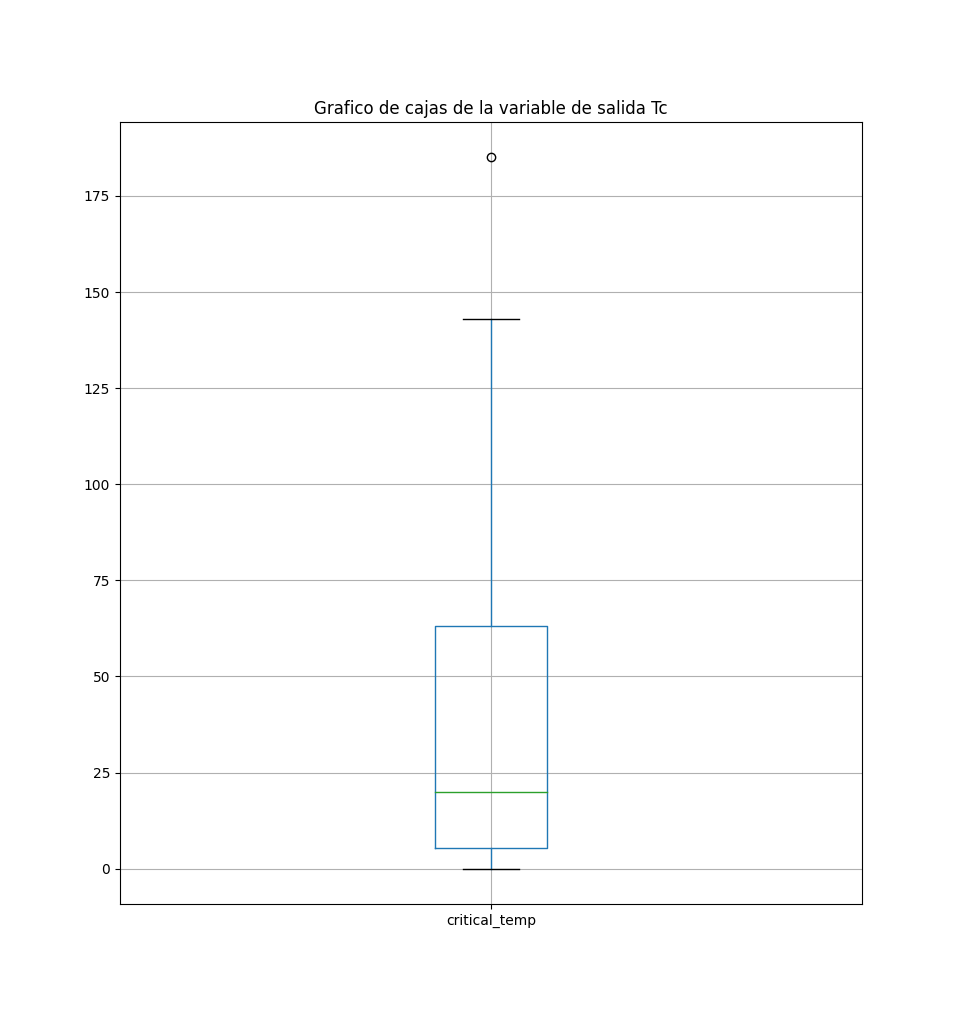
\includegraphics[width=0.5\textwidth]{output_var_boxplot}
    \caption{Boxplot de la temperatura crítica}
\end{figure}

La caja del gráfico muestran los extremos de los extremos que fijan el percentil 25 y 75. Por tanto, podemos ver que nuestros datos de entrada están muy acumulados en valores de salida bajos. Es decir, la mayoría de datos con los que trabajamos están asociados a superconductores con un $T_c$ bajo, y por tanto menos interesantes. Esto mismo se comenta en el paper original, en la figura 4 \cite{original_paper_reg:paper}.

Por tanto, debemos preservar estos \emph{outliers} en la variable de salida, pues son precisamente los datos que nos interesa predecir. Podríamos intentar solucionar este desbalanceo eliminando datos en la parte de mayor acumulación (datos de baja temperatura $T_c$). Sin embargo, a vista de lo desplazada que está la caja del gráfico, eliminaríamos demasiados datos, con lo que seguramente no mejoraríamos el rendimiento de la función aprendida. Además, nuestro objetivo no es aprender bien la función para superconductores con $T_c$ alto (aunque sean los más interesantes), sino aprender bien la función $f$ que ya hemos descrito anteriormente.

\pagebreak
\subsection{Preprocesado de los datos}

\subsubsection{Eliminación de outliers}

Antes de realizar normalización, debemos eliminar los \emph{outliers}. Estos son aquellos valores que están a una distancia de la media de más de 3 veces la desviación típica. Tenemos distintas características por cada dato, así que definimos los \emph{outliers} como aquellas filas que, en alguna de las variables que definen las columnas, se desvían como ya hemos especificado. Podríamos haber optado por técnicas que detectasen \emph{outliers} basándonos en más de una variable, pero por simplicidad, seguimos el procedimiento ya indicado. La opción multivariable preserva más datos, pero tenemos un \emph{dataset} lo suficientemente grande como para permitir el borrar más filas.

En nuestro caso, por ser menos restrictivos, establecemos el límite en 4 veces la desviación típica.

Todo esto está fundamentado en que, en una distribución normal, el $99.74\%$ de los datos se encuentran en el intervalo $[\mu - \sigma, \mu + \sigma]$. Al tener una gran cantidad de datos, por el teorema central del límite, podemos suponer que nuestra distribución de datos se aproxima a una distribución normal (multivariante al tener varias variables).

Además, hacemos esto antes de estandarizar, pues para estandarizar, usamos los estadísticos media y desviación típica, que son muy sensibles a los valores \emph{outliers} \cite{scikit_scale_with_outliers:online}. También afectan los \emph{outliers} al procedimiento de \emph{PCA}, pues se basa en estadísticos altamente afectados por dichos \emph{outliers} \cite{pca_medium:online}.

Previamente hemos justificado que no vamos a borrar \emph{outliers} respecto a la variable de salida.

El código que borra los outliers se encuentra en la función \lstinline{remove_outliers}. Usamos una orden de acceso de la librería \lstinline{pandas} en la que usamos el estadístico \lstinline{zscore}, de la librería \lstinline{scipy}. Este valor \lstinline{zscore} lo que mide es el número de desviaciones típicas en las que un punto dista de la media de la variable aleatoria, es decir:

$$z_{score}(x) := \frac{x - \mu}{\sigma}$$

Borramos aquellos valores que, en alguna variable aleatoria columna, tengan un valor absoluto de \lstinline{zscore} mayor o igual que 4.

Tras ejecutar el eliminado de \emph{outliers}, eliminamos el 8.78\% de los datos. Teniendo en cuenta la gran cantidad de datos de los que disponemos, junto al hecho de que en \cite{original_paper_reg:paper} comentan los autores que se quedan con el 67\% de los datos originales, para acabar con un \emph{dataset} de calidad, queda justificada esta pérdida de datos en pro de un conjunto de datos más limpio y de calidad.

En este punto nos preocupamos de haber eliminado, sin fijarnos en la variable de salida, filas con valores de salida interesantes o que desbalanceen aún más el conjunto de datos. Sin embargo, computamos unas cuantas estadísticas de las filas eliminadas, respecto de la columna de salida $T_c$. La media de los datos eliminados es 12.82, y la desviación típica es 22.34. Por tanto estamos eliminando mayoritariamente filas con $T_c$ bajos, así que no vemos que estemos introduciendo aún más desbalanceo.

\subsubsection{Principal Component Analysis}

Con esta técnica buscamos reducir la dimensionalidad de nuestro conjunto de datos, manteniendo el máximo de la variabilidad original (que es lo que nos permite llevar a cabo un proceso de aprendizaje).

Buscamos una base ortonormal de un espacio $\mathbb{R}^{\hat{d}}$ donde $\hat{d} << d$, es decir, el nuevo espacio euclídeo tiene una dimensión mucho menor que el espacio original. Todo esto gracias a calcular los valores propios de la matriz de covarianzas del conjunto de datos original \cite{pca_wikipedia:online} \cite{pca_article:online}. Con ello, y usando propiedades de vectores y espacios propios, expresamos en espacio con vectores que están linealmente incorrelados.

Además, esta técnica devuelve los vectores de la base ordenados según la varianza que explican del conjunto de datos original.

En nuestro caso, esta trasnformación del espacio la realizamos gracias a la función \lstinline{apply_PCA}. Podemos especificar el número de variables con el que nos queremos quedar, como el porcentaje de varianza que queremos alcanzar. Notar que pasamos como parámetro el conjunto de test. Este conjunto de test \textbf{no se usa para calcular la transformación}, solo se pasa para aplicar la misma transformación calculada, de nuevo, exclusivamente usando los datos del conjunto de entrenamiento.

Cuando buscamos un 95\%, con 3 componentes parece que es suficiente. Esto parece tener sentido, pues tenemos 8 variables dependientes de los átomos, que ya de por sí estarán en cierto grado correladas, y 10 estadísticas moleculares, que podemos suponer altamente correladas. Sin embargo, quedarnos de un conjunto de 81 variables con solo 3 parece excesivo. Por tanto tomamos arbitrariamente la decisión de quedarnos con 10 columnas, el 12.3\% de las variables. Esto porque ya hemos comentado que tenemos 8 variables atómicas, y añadimos dos variables más para tener algo de margen con las estadísticas moleculares.

Quedándonos con 10 variables obtenemos un  99.950\% de la variabilidad original explicada.

Un detalle destacable es que antes de aplicar \emph{PCA} no estandarizamos el conjunto de datos, pues esto produce peores resultados. Esto tiene sentido pues \emph{PCA} se basa en correlación de variables, que es alterada cuando hacemos estandarización basada en una única variable a la vez (como veremos más adelante).

Las estadísticas del conjunto de datos tras la transformación se refleja en la siguiente tabla:

\begin{table}[H]
\resizebox{\columnwidth}{!}{%
\begin{tabular}{|c|c|c|c|c|c|c|c|c|}
\hline
    \textbf{Columna}                             &    \textbf{mean}&       \textbf{median}&           \textbf{var}&          \textbf{sdt}&         \textbf{min}&           \textbf{max}&          \textbf{p25}&          \textbf{p75}  \\
\hline

0  &   -2.28e-13& -3464.06&  4.79e+7&  6923.94&  -8121.31&  39063.60& -4783.59&  3770.72 \\
1  &    2.05e-12&    10.68&  2.30e+7&  4798.68& -11192.14&  18391.68& -2274.11&  1340.20 \\
2  &   -3.15e-13&   -17.09&  3.82e+6&  1956.17& -10235.37&  14248.53&  -774.02&   684.64 \\
3  &   -6.75e-13&    98.48&  8.06e+5&   897.95&  -3794.20&   7688.15&  -574.11&   512.52 \\
4  &   -8.79e-13&    93.72&  6.67e+5&   816.88&  -4432.94&   5548.37&  -539.45&   479.13 \\
5  &    6.42e-13&   -82.54&  4.10e+5&   641.01&  -2259.87&   4500.24&  -273.61&   286.83 \\
6  &   -4.11e-13&    -3.76&  1.16e+5&   340.72&  -1790.88&   2917.67&  -182.77&   175.26 \\
7  &   -9.67e-14&   -49.58&  6.11e+4&   247.32&  -1530.81&   2782.81&  -153.15&   135.49 \\
8  &    6.75e-15&     7.06&  3.34e+4&   182.90&   -779.76&    855.90&   -79.61&   111.87 \\
9  &    1.09e-13&    -8.45&  1.61e+4&   127.25&   -510.65&   1033.12&   -73.78&    66.47 \\

\hline
    \end{tabular}
    }
    \caption{Estadísticas de las \emph{features} tras aplicar \emph{PCA}}
\end{table}

Es claro que no controlamos la transformación, por tanto no tenemos interpretación de lo que representa cada columna. También es claro que tenemos desviaciones típicas en órdenes de magnitud distintas y rangos (mínimo y máximo) completamente dispares. Por tanto, tanto como con el conjunto de datos original como en el conjunto tras aplicar \emph{PCA}, es necesario realizar una estandarización o normalización de los datos.

\subsubsection{Estandarización}

En este proceso, buscamos que las variables aleatorias de nuestro conjunto de datos queden con media cero y desviación típica uno. Este proceso no hace que las variables estén en un rango de valores similares, sin embargo, en este problema de regresión no parece ser importante. No usamos técnicas basadas en proximidad como \emph{nearest neighbour} o \emph{SVM}, en las que una normalización sería más adecuada la normalización \cite{normalization_vs_standarization:online}. En normalización conseguríamos que todas las variables estuviesen en el rango $[0, 1]$.

En estandarización, aplicamos la siguiente operación a todas las variables aleatorias que conforman nuestro conjunto de datos:

$\mathbb{X'} = \frac{\mathbb{X} - \mu}{\sigma}$

El código usado para estandarizar se encuentra en \lstinline{standarize_dataset}. De nuevo, recibe como parámetro el conjunto de test. Este conjunto no se usa para calcular la transformación que representa la estandarización. Este cálculo solo toma información de los datos de entrenamiento. Por tanto, sobre el conjunto de test, solo se aplica la misma transformación.

En dicho código usamos la clase \lstinline{StandarScaler} de \lstinline{sklearn}, que hace justo lo que hemos especificado \cite{sklearn_std_scaler:online}.

Aplicamos estandarización tanto al conjunto original de datos, al que solo hemos borrado outliers, como al conjunto que queda tras aplicar \emph{PCA}.

En dicho código se puede observar que no estamos estandarizando la variable de salida, pues esto no tiene sentido. En datos no vistos en el entrenamiento, nos llegan variables de entrada pero no de salida. Así que la predicción debe hacerse en el conjunto aleatorio que representa la variable aleatoria de salida original.

Mostramos algunos de los datos, no todos pues no tiene mayor interés, de ambos conjuntos de datos tras estandarizar.


\begin{table}[H]
\centering
\begin{tabular}{|c|c|c|c|c|c|c|c|c|}
\hline
\textbf{name}&                \textbf{mean}&     \textbf{median}&          \textbf{var}&        \textbf{sdt}&       \textbf{min}&         \textbf{max}&       \textbf{p25}&        \textbf{p75} \\
\hline
0&               -1.37-17&  -0.50&     1.00&   1.00& -1.17&    5.64& -0.69&   0.54 \\
1&               -1.67-17&   0.00&     1.00&   1.00& -2.33&    3.83& -0.47&   0.27 \\
2&               -3.44-18&  -0.00&     1.00&   1.00& -5.23&    7.28& -0.39&   0.35 \\
\hline
    \end{tabular}
    \caption{Conjunto de datos tras aplicar \emph{PCA} y \emph{estandarización}}
\end{table}

\begin{table}[H]
\centering
\begin{tabular}{|c|c|c|c|c|c|c|c|c|}
\hline
\textbf{name} &                                      \textbf{mean} &    \textbf{median} &       \textbf{var} &       \textbf{sdt} &       \textbf{min} &       \textbf{max} &       \textbf{p25} &       \textbf{p75} \\
\hline
numberof\_elements              &  1.95e-16& -0.07&  1.00&  1.00& -2.15&  3.38& -0.77&  0.61 \\
meanatomic\_mass                & -5.66e-17& -0.08&  1.00&  1.00& -2.71&  4.09& -0.50&  0.43 \\
wtdmean\_atomic\_mass            &  3.29e-17& -0.36&  1.00&  1.00& -1.98&  4.05& -0.62&  0.39 \\
gmeanatomic\_mass               & -2.81e-16& -0.15&  1.00&  1.00& -2.12&  4.44& -0.43&  0.22 \\
\ldots &  \ldots & \ldots & \ldots & \ldots &  \ldots & \ldots & \ldots & \ldots \\
wtdrange\_Valence               & -4.75e-17& -0.42&  1.00&  1.00& -1.50&  5.59& -0.57&  0.44 \\
stdValence                     & -3.22e-16& -0.08&  1.00&  1.00& -1.72&  4.42& -0.76&  0.75 \\
wtdstd\_Valence                 &  7.12e-17& -0.38&  1.00&  1.00& -1.47&  5.08& -0.80&  0.75 \\
\hline
    \end{tabular}
    \caption{Conjunto de datos sin aplicar \emph{PCA} tras la \emph{estandarización}}
    \label{tabla_sin_pca}
\end{table}

En ambas tablas vemos que acabamos con desviación típica 1 y media prácticamente cero (notar que tenemos valores en órdenes de magnitud de $10^{-16}$ o $10^{-17}$, es decir, prácticamente cero). Aunque esta técnica de escalado no se centre en normalizar el rango de valores, si que hace que los rangos se normalicen algo. Por ejemplo, en la \emph{Tabla \ref{tabla_sin_pca}. \nameref{tabla_sin_pca}}, el valor de \emph{meanatomic\_mass} se mueve ahora en un rango $[-2.71, 4.09]$, mientras que en la \emph{Tabla \ref{Tabla con los estadísticos de las features}. \nameref{Tabla con los estadísticos de las features}} podemos ver que se movía en un rango $[6.94, 208.98]$. Así que aunque no estemos explícitamente preocupándonos por el rango de las variables, sí que estamos haciendo que no sean rangos tan amplios ni rangos tan dispares entre distintas variables.

\pagebreak
\subsection{Selección del modelo}

\subsubsection{Selección de la métrica de error}

=> Métrica de error -> error cuadrático medio
=> No uso error medio -> con error cuadrático medio se castigan más los outliers. Son funciones con una derivada mas sencilla a la hora de minimizar
=> El ECM es de los pocos errores que hemos visto a la hora de aplicar regresión, mientras que en clasificación teníamos más variedad para elegir
=> No usamos SGDRegressor porque tenemos la suficiente potencia de cómputo para usar Lasso, Ridge y LinearModel. Cuando el ordenador no puede más, es por la transformacion polinomica
=> Asi que elijo Linear normal, ridge y Lasso para CV etapa1
    => Laso es interesante porque favorece que muchos coeficientes sean cero. Ridge favorece pesos pequeños pero no cero. Interesante para quitar terminos del polynomial fit que no me interesan

\subsubsection{Modelos candidatos}

A la hora de seleccionar modelos disponemos de:

\begin{itemize}
    \item Ajustar un hiperplano
\end{itemize}

Así que en realidad a la hora de escoger un modelo debemos escoger la trasnsformación de los datos sobre la que ajustaremos un hiperparámetro. También deberemos escoger el regularizador

\subsubsection{\emph{Cross-Validation}, primera etapa}

=> Explicar que he hecho en codigo, seleccion de lambda fijado por mi, la metrica de error negativa, las transformaciones que hemos realizado...
=> Comentar que en lasso saltan errores, y se vuelve a intentar asignando distintos valores o mas iteraciones -> No estoy muy seguro de esta politica
=> Cuando uso No PCA, antes hago una normalizacion de los datos

Los resultados de \emph{Cross Validation} se resumen en la siguiente tabla:

==> Quitar tabularx porque va mal
\begin{table}[H]
\begin{tabularx}{\textwidth}{|X|X|X|X|X|X|}
    \hline
    \textbf{Modelo} & \textbf{PCA \/ No PCA}& \textbf{Orden de la transformación polinómica} & \textbf{Valor medio} & \textbf{Valor mínimo} & \textbf{Valor máximo} \\
    \hline
    Lineal & PCA & 1 & -572.19 & -601.20 & -535.89 \\
    Lineal & PCA & 2 & -431.65 &-476.37 & -412.32 \\
    Lineal & PCA & 3 &-350.63 &-386.93 & -326.35 \\
    Lineal & PCA & 4 & -2470.37 &-15358.09 & -283.22 \\
    Ridge  & PCA & 1 &-572.15 &-609.16 & -541.24 \\
    Ridge  & PCA & 2 & -431.82 &-472.09 & -404.95 \\
    Ridge  & PCA & 3 & -348.22 &-363.54 & -332.83 \\
    Ridge  & PCA & 4 & -2126.95 &-14843.43 & -333.92 \\
    Lasso  & PCA & 1 & -572.15 &-634.92 & -549.44 \\
    Lasso  & PCA & 2 & -432.08 &-459.59 & -413.28 \\
    Lasso  & PCA & 3 & -358.46 &-382.28 & -335.32 \\
    Lasso  & PCA & 4 & -361.25 &-592.61 & -304.22 \\
    Lineal & No PCA & 1 & -310.50 &-322.55 & -282.40 \\
    Ridge  & No PCA & 1 & -310.77 &-335.69 & -292.88 \\
    Lasso  & No PCA & 1 & -328.42 &-355.69 & -310.94 \\
    \hline
\end{tabularx}
    \caption{Resultados de \emph{Cross Validation}, primera fase}
\end{table}

=> Por tanto, escogemos no aplicar PCA
=> Por tanto, aunque la mejor media la da Linea No PCA, usamos Ridge No PCA, pues difieren solo en media en 0.27 ECM y no hemos jugado con el parametro de regularizacion, asi que parece que vamos a poder mejorar aun mas el performance del modelo
    -> Ademas, ridge es más estable a vista del Maximo Minimo en un intervalo de menor longitud
=> Puede tener sentido no aplicar PCA -> $N \geq d_{VC} * 10 \rightarrow d_{VC} \leq 1600$

\subsubsection{\emph{Cross-Validation, segunda etapa}}

=> Elegimos el dataset original sin PCA ni transformaciones polinomicas
=> Regularizador ridge
=> Rango de valores para lambda: $[10^-6 ... 10^-1, 1, 2]$ -> basado en ??

=> Se resume en la siguiente tabla:

=> Va mal tabularx
\begin{table}[H]
\begin{tabularx}{\textwidth}{|X|X|X|X|}
    \hline
    \textbf{Lambda} & \textbf{Valor medio} & \textbf{Valor mínimo} & \textbf{Valor máximo} \\
    \hline
    1e-07 & -310.50 &  -322.55 & -282.40 \\
    1e-06 & -310.50 &  -322.55 & -282.40 \\
    5e-06 & -310.55 &  -335.61 & -272.69 \\
    1e-05 & -310.77 &  -335.67 & -292.98 \\
    0.0001 & -310.74 &  -343.24 & -291.18 \\
    0.001 & -310.79 &  -348.74 & -287.12 \\
    0.01 & -310.58 &  -356.06 & -283.69 \\
    0.1 & -310.75 &  -324.71 & -298.66 \\
    1 & -310.99 &  -335.25 & -276.35 \\
    2 & -311.13 &  -329.18 & -291.28 \\
    5 & -311.90 &  -336.92 & -287.86 \\
    \hline
\end{tabularx}
    \caption{Resultados de \emph{Cross Validation}, segunda fase}
\end{table}

=> A vista de esto, usamos $\lambda = 10^{-7}$


==> TODO -- en algun commento comentar que estamos usando unos baselines
\pagebreak
\section{Problema de clasificación}

\pagebreak

% Bibliografia
\bibliography{./References}
\bibliographystyle{ieeetr}

\end{document}
